\documentclass{beamer}
\usepackage{amsmath,amsbsy,amsopn,amstext,amsfonts,amssymb}
\usepackage{isomath}
\usepackage{ulem}
%\linespread{1.6}  % double spaces lines
\usepackage{graphicx}
\usepackage{subfigure}
\usepackage{color}
\usepackage{optidef}  % define optimization problems
\usepackage{multicol}  % multiple columns
\usepackage{listings} % for python code
\usepackage{mathrsfs}

\usepackage{polynom}
\newcommand{\adj}{\mathrm{adj}}
\newcommand{\constrainedmin}[3]{
		\begin{mini*}|s|
		{#2}{#1}{}{}
		\addConstraint{#3}
		\end{mini*}
}

\newcommand{\rwbcomment}[1]{{\color{blue}RWB:#1}}
\newcommand{\defeq}{\stackrel{\triangle}{=}}
\newcommand{\abs}[1]{\left|#1\right|}
\newcommand{\norm}[1]{\left\|#1\right\|}
\newcommand{\iprod}[1]{\left<#1\right>}
\newcommand{\ellbf}{\boldsymbol{\ell}}
\newcommand{\nubf}{\boldsymbol{\nu}}
\newcommand{\mubf}{\boldsymbol{\mu}}
\newcommand{\abf}{\mathbf{a}}
\newcommand{\bbf}{\mathbf{b}}
\newcommand{\cbf}{\mathbf{c}}
\newcommand{\dbf}{\mathbf{d}}
\newcommand{\ebf}{\mathbf{e}}
\newcommand{\fbf}{\mathbf{f}}
\newcommand{\gbf}{\mathbf{g}}
\newcommand{\hbf}{\mathbf{h}}
\newcommand{\ibf}{\mathbf{i}}
\newcommand{\jbf}{\mathbf{j}}
\newcommand{\kbf}{\mathbf{k}}
\newcommand{\lbf}{\mathbf{l}}
\newcommand{\mbf}{\mathbf{m}}
\newcommand{\nbf}{\mathbf{n}}
\newcommand{\obf}{\mathbf{o}}
\newcommand{\pbf}{\mathbf{p}}
\newcommand{\qbf}{\mathbf{q}}
\newcommand{\rbf}{\mathbf{r}}
\newcommand{\sbf}{\mathbf{s}}
\newcommand{\tbf}{\mathbf{t}}
\newcommand{\ubf}{\mathbf{u}}
\newcommand{\vbf}{\mathbf{v}}
\newcommand{\wbf}{\mathbf{w}}
\newcommand{\xbf}{\mathbf{x}}
\newcommand{\ybf}{\mathbf{y}}
\newcommand{\zbf}{\mathbf{z}}
\newcommand{\Jbf}{\mathbf{J}}
\newcommand{\Acal}{\mathcal{A}}
\newcommand{\Bcal}{\mathcal{B}}
\newcommand{\Lcal}{\mathcal{L}}
\newcommand{\Ncal}{\mathcal{N}}
\newcommand{\Rcal}{\mathcal{R}}
\definecolor{darkolivegreen}{rgb}{0.33, 0.42, 0.18}

\makeatletter
\newenvironment<>{proofstart}[1][\proofname]{%
    \par
    \def\insertproofname{#1\@addpunct{.}}%
    \usebeamertemplate{proof begin}#2}
  {\usebeamertemplate{proof end}}
\newenvironment<>{proofcont}{%
  \setbeamertemplate{proof begin}{\begin{block}{}}
    \par
    \usebeamertemplate{proof begin}}
  {\usebeamertemplate{proof end}}
\newenvironment<>{proofend}{%
    \par
    \pushQED{\qed}
    \setbeamertemplate{proof begin}{\begin{block}{}}
    \usebeamertemplate{proof begin}}
  {\popQED\usebeamertemplate{proof end}}
\makeatother

\title{ECEn 671: Mathematics of Signals and Systems}
\author{Randal W. Beard}
\institute{Brigham Young University}
\date{\today}

\begin{document}

%-------------------------------
\begin{frame}
	\titlepage
\end{frame}



%%%%%%%%%%%%%%%%%%%%%%%%%%%%%%%%%%%%%%%%%%%%%%%%%%%%%%%%%%%%%%%%%
\section{Quadratic Forms}
\frame{\sectionpage}

%----------------------------------
\begin{frame}\frametitle{Quadratic Forms}
	\begin{definition}
		A real square matrix is \underline{symmetric} if $A^\top =A$	
	\end{definition}
	
	\begin{definition}
		A real square matrix is \underline{skew-symmetric} if $A^\top  = -A$
	\end{definition}
\end{frame}

%----------------------------------
\begin{frame}\frametitle{Quadratic Forms}
	\begin{lemma}
		Any real square matrix $B\in\mathbb{R}^{n\times n}$ can be written as
		\[ 
			B = B_s + B_{ss} 
		\]
		where $B_s$ is symmetric and $B_{ss}$ is skew-symmetric.
	\end{lemma}
	
	\begin{proof}
		\begin{align*}
			B &= \frac{B + B^\top }{2} + \frac{B - B^\top }{2} 
			  \defeq  B_s + B_{ss} 
		\end{align*}
		where
		\begin{align*}
			B_s^\top  &= \left(\frac{B + B^\top }{2}\right)^\top  
			      = \frac{B^\top  - B}{2} = \frac{B + B^\top }{2} 
			      = B_s \\
			B_{ss}^\top  &= \left(\frac{B-B^\top }{2}\right)^\top  
			         = \frac{B^\top -B}{2} 
			          = -\left(\frac{B-B^\top }{2}\right) 
			         = -B_{ss} 
		\end{align*}
	\end{proof}
\end{frame}

%----------------------------------
\begin{frame}\frametitle{Quadratic Forms}
	\begin{lemma}
		For any real square matrix $A$ and for all $y$
		\[ 
			y^\top Ay = y^\top A_sy 
		\]
		where $A_s$ is the symmetric part of $A$.
	\end{lemma}
	
	\begin{proof}
	\[ 
		y^\top Ay = y^\top A_sy + y^\top A_{ss}y 
	\]
	but
	\[
		y^\top A_{ss}y = y^\top \left(\frac{A-A^\top }{2}\right)y 
		           = \frac{1}{2}y^\top Ay - \frac{1}{2}y^\top A^\top y.
	\]
	But since
	\[
		y^\top A^\top y = (y^\top A^\top y)^\top  
		        = y^\top Ay 
		        \implies y^\top A_{ss}y = 0.
	\]		
	\end{proof}
\end{frame}

%----------------------------------
\begin{frame}\frametitle{Quadratic Forms}
	\begin{definition}
		A \underline{quadratic form} of a real square matrix $A$ is $Q_A(y) = \ybf^\top A \ybf$.		
	\end{definition}
	
	w.l.o.g. $A$ can be assumed to be symmetric.  If not, we can always limit our attention to the symmetric part of $A$ since
	\[ 
		\ybf^\top A \ybf = \ybf^\top A_s \ybf. 
	\]
	Quadratic forms show up in numerous places.	For example, the pdf for a Gaussian random variable is 
	\[
	p(\xbf) = \frac{1}{\sqrt{(2\pi)^n\det(\Sigma)}}\exp\left(-\frac{1}{2}(\xbf-\mubf)^\top \Sigma^{-1} (\xbf-\mubf)\right).
	\]	
\end{frame}

%----------------------------------
\begin{frame}\frametitle{Quadratic Forms}
	\begin{example}
		Let 
		\[
			Q_A(\ybf) = \ybf^\top \begin{pmatrix} 1 & 0 \\ 0 & 1 \end{pmatrix} \ybf = y_1^2 + y_2^2 = c
		\]
		\begin{center}
			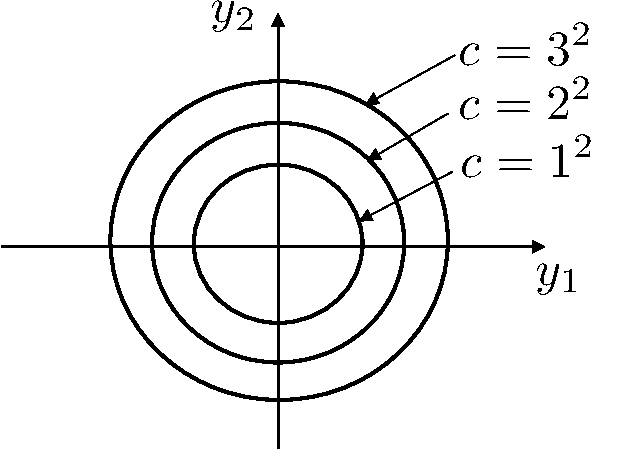
\includegraphics[width=0.5\textwidth]
				{figures/chap6_level_curve_circle}	
		\end{center}
		The level curves of $Q_A(\ybf)$ are circles of radius $\sqrt{c}$.
	\end{example}
\end{frame}


%----------------------------------
\begin{frame}\frametitle{Quadratic Forms}
	\begin{example}
	Consider the quadratic equation
	\[
		f(x) = 2y_1^2 + 3 y_1 y_2 + 4 y_2^2,
	\]	
	and note that
	\begin{align*}
		f(x) 
			&= 2y_1^2 + 3 y_1 y_2 + 4 y_2^2 \\
		 	&= 	\begin{pmatrix}
 					y_1 & y_2 
 				\end{pmatrix}
 				\begin{pmatrix}
 					2y_1 + \frac{3}{2} y_2 \\
 					4y_2 + \frac{3}{2} y_1
 				\end{pmatrix} \\
 		 	&= 	\begin{pmatrix}
 					y_1 & y_2 
 				\end{pmatrix}
 				\begin{pmatrix}
 					2 & \frac{3}{2} \\
 					\frac{3}{2} & 4 
 				\end{pmatrix} 
 				\begin{pmatrix}
 					y_1 \\ y_2	
 				\end{pmatrix} \\
 			&= \ybf^\top A \ybf
	\end{align*}
	\end{example}
	
	Any quadratic equation in $n$ variables can be written in the form $\ybf^\top A \ybf$.
	
\end{frame}


%----------------------------------
\begin{frame}\frametitle{Quadratic Forms}
	By the spectral theorem, $A$ is diagonalizable.  In other words, there exists an invertible $U$ so that 
	$A = U\Lambda U^\top $.
	
	\vfill
	
	From Moon Lemma 6.2 the eigenvalues are real so we can order them as
	\[ 
		\Lambda 
			= \begin{pmatrix}
	    		\lambda_1\\
	    		& \lambda_2\\
	    		& & \ddots\\
	    		& & & \lambda_n
	  		   \end{pmatrix}
	\]
	with
	\[
	  	\lambda_1 \geq \lambda_2 \geq \ldots \geq \lambda_n.
	\]
\end{frame}

%----------------------------------
\begin{frame}\frametitle{Quadratic Forms}
	\begin{lemma}
		Level curves of the quadratic form 
		\[
			Q_A(x-x_0) = (x-x_0)^\top A(x-x_0) = c
		\]
		are hyper-ellipsoids with the length of the axes given by $\frac{1}{\sqrt{\lambda_i}}$.	
	\end{lemma}
	\begin{proofstart}
		Let $z = U^\top y$ then
		\begin{align*}
		 Q_A(y) &= y^\top Ay= y^\top U\Lambda U^\top y = z^\top \Lambda z \\
		 		&= \begin{pmatrix}
		     			z_1 & \cdots & z_n
			   	   \end{pmatrix}
			   	   \begin{pmatrix}
		     			\lambda_1 & & 0\\
		     			& \ddots\\
		     			0 & & \lambda_n
		   			\end{pmatrix}
		   			\begin{pmatrix}
		    			z_1 \\ \vdots \\ z_n
		  			\end{pmatrix} \\
		  		&= \lambda_1 z_1^2 + \dots + \lambda_n z_n^2
		\end{align*}
	\end{proofstart}
\end{frame}

%----------------------------------
\begin{frame}\frametitle{Quadratic Forms}
	\begin{proofcont}
		Note that in the variable $z$, the quadratic form is an ellipsoid:
		\[ 
			Q_A(\ybf)= (\sqrt{\lambda_1})^2z_1^2 + (\sqrt{\lambda_2})^2z_2^2 + \cdots + (\sqrt{\lambda_n})^2z_n^2 = 1 
		\]
		or
		\[ 
			Q_A(\ybf)= \frac{z_1^2}{\left(\frac{1}{\sqrt{\lambda_1}}\right)^2} + \frac{z_2^2}{\left(\frac{1}{\sqrt{\lambda_2}}\right)^2} + \cdots + \frac{z_n^2}{\left(\frac{1}{\sqrt{\lambda_n}}\right)^2} = 1
		\]
		Either of these are the general equation for an ellipsoid with minor axis 
		$\ebf_1 = 	\begin{pmatrix}
						1 & 0 & \cdots & 0 
				  	\end{pmatrix}^\top$ 
		and major axis 
		$\ebf_n = 	\begin{pmatrix} 
						0 & \cdots & 0 & 1
					\end{pmatrix}^\top$
	\end{proofcont}
\end{frame}

%----------------------------------
\begin{frame}\frametitle{Quadratic Forms}
	\begin{columns}
		\begin{column}{0.6\textwidth}
			Note that along $\ebf_1$, the stretching is
			\[ 
				(\sqrt{\lambda_1})^2z_1^2 = 1 \Rightarrow z_1 = \frac{1}{\sqrt{\lambda_1}} 
			\]
			\begin{center}
				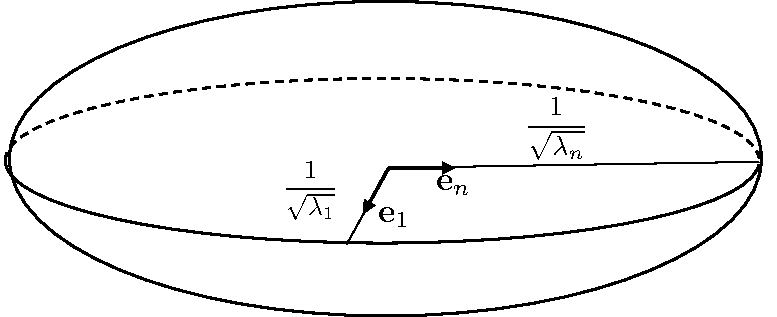
\includegraphics[width=0.99\textwidth]{figures/chap6_quadratic_form_1}
			\end{center}
		\end{column}
		\begin{column}{0.5\textwidth}
			In the original space, what is $\ebf_1$?
			\begin{align*}
				\ebf_1 &= U^\top \ybf 
				    = \begin{pmatrix}
			    		\ubf_1^\top \\
			    		\vdots\\
			    		\ubf_n^\top 
			  		  \end{pmatrix}\ybf \\
			  		&= \begin{pmatrix}
			    		\ubf_1^\top \ybf\\
			    		\vdots\\
			    		\ubf_n^\top \ybf
			  		  \end{pmatrix} 
			  		= \begin{pmatrix}
			    		1\\0\\\vdots\\0
			  		  \end{pmatrix}.
			\end{align*}
			Therefore $\ybf = \ubf_1$ since $U$ is orthogonal.
			
			i.e. $\ubf_i = U \ebf_i$	.
		\end{column}	
	\end{columns}
\end{frame}

%----------------------------------
\begin{frame}\frametitle{Quadratic Forms}
	Therefore the major axis is given by the eigenvector associated with the smallest eigenvalue, and the minor axis is given by the eigenvector associated with the largest eigenvalue.
	
	\vfill
	
	{\color{blue} Question:}  What is the geometric picture associated with
	\[
		(x-x_0)^\top A(x - x_0) = c 
	\]
	where $c$ is a constant and $A$ is symmetric and positive definite?
	
	\vfill
	
	{\color{blue} Answer:}  An ellipsoid of radius $\sqrt{c}$ centered at $x_0$ with axes along the eigenvectors of $A$ and stretching along each axis given by $\displaystyle \frac{1}{\sqrt{\lambda_i}}$.
\end{frame}

%----------------------------------
\begin{frame}\frametitle{Quadratic Forms}
	{\color{blue}Question:}  
	What if we would like to maximize
	\[ 
		Q_A(y) = y^\top Ay \text{ where } \norm{y} = 1.
	\]
	Which axis provides the most bang-for-the-buck?
	
	\vfill
	
	{\color{blue}Answer:} The \underline{major} axis!  i.e. the axis associated with the largest eigenvalue.
	
\end{frame}

%----------------------------------
\begin{frame}\frametitle{Quadratic Forms}
	Rather than drawing
	\[ 
		\lambda_1 z_1^2 + \lambda_2 z_2^2 + \cdots + \lambda_n z_n^2 = 1 
	\]
	which is
	\begin{center}
		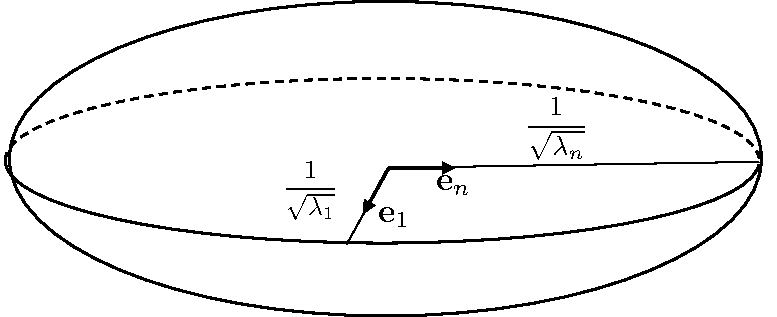
\includegraphics[width=0.5\textwidth]{figures/chap6_quadratic_form_1}
	\end{center}
	lets draw the mapping of the unit circle through $\ybf^\top A\ybf$
	i.e.
	\[ 
		\{ \norm{\ybf}=1 \} 
			\overset{Q_A(\ybf)}{\longrightarrow} 
		\{ \ybf^\top A \ybf \}
	\]
	\begin{center}
		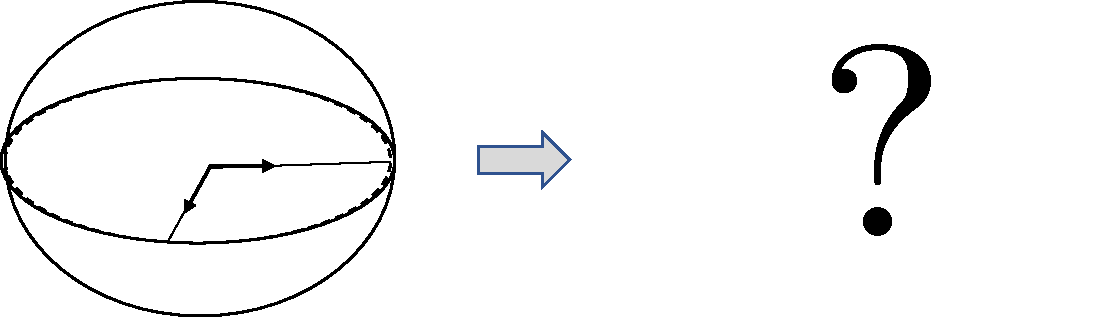
\includegraphics[width=0.5\textwidth]
			{figures/chap6_mapping_1}
	\end{center}
\end{frame}

%----------------------------------
\begin{frame}\frametitle{Quadratic Forms}
	If $A=A^\top $ then $A=U\Lambda U^\top $ where $U$ is orthogonal, i.e., $UU^\top =U^\top U=I$.
	Then
	\begin{align*}
		\max_{\norm{\ybf}=1} \ybf^\top  A \ybf 
			&= \max_{\norm{\ybf}=1} \ybf^\top  U \Lambda U^\top  \ybf.	
	\end{align*}
	
	\vfill

	Let $\zbf=U^\top  \ybf$ and note that $\norm{\zbf}=\norm{U^\top  \ybf} = \norm{\ybf}$ since $U$ is orthogonal.
	Then 
	\begin{align*}
		\max_{\norm{\ybf}=1} \ybf^\top  U \Lambda U^\top  \ybf 
			&= \max_{\norm{\zbf}=1} \zbf^\top  \Lambda \zbf \\
			&= \max_{\norm{\zbf}=1} \left( \lambda_1 z_1^1 + \lambda_2 z_2^2 + \cdots + \lambda_n z_n^2 \right)	
	\end{align*}
	where $\Lambda$ is arranged such that
	\[
	\lambda_1 \geq \lambda_2 \geq \cdots \geq \lambda_n.
	\]
\end{frame}

%----------------------------------
\begin{frame}\frametitle{Quadratic Forms}
	The maximum is therefore 
	\[
	\zbf^\ast = \begin{pmatrix} 1 & 0 & \vdots & 0 \end{pmatrix}^\top
	\]
	where it is clear that $\norm{\zbf}=1$.
	
	Furthermore
	\[
		\max_{\norm{\zbf}=1} \zbf^\top  \Lambda \zbf = \lambda_1,
	\]
	which implies that
	\[
	\ybf^\ast = U\zbf^\ast = \begin{pmatrix} \ubf_1 & \cdots & \ubf_n \end{pmatrix} \begin{pmatrix} 1 \\ 0 \\ \vdots \\ 0 \end{pmatrix} = \ubf_1.
	\]	
\end{frame}

%----------------------------------
\begin{frame}\frametitle{Quadratic Forms}
	This mapping also forms an ellipsoid but with a different effect.
	
	Let $\ybf = \ubf_1 \implies \norm{\ybf} = 1 $ to get
	\[ 
		Q_A(\ybf) = \lambda_1 
	\]
	
	\vfill
	
	{\color{blue}Question:} 
	Is it possible to pick a $\hat{\ybf}$ where $\norm{\hat{\ybf}} = 1$ such that 
	\[
		Q_A(\hat{\ybf}) > Q_A(\ubf_1)?
	\]
	
	\vfill
	
	{\color{blue}Answer:} No.
	
\end{frame}

%----------------------------------
\begin{frame}\frametitle{Quadratic Forms}
	{\color{blue}Explanation:}
	Recall that $\lambda_1 \geq \lambda_2 \geq \ldots \geq \lambda_n$ and $\norm{\hat{\ybf} } = y_1^2 + \cdots + y_n^2 = 1$.
	
	\vfill
	
	Therefore
	\begin{align*}
		Q_A(\hat{\ybf}) 
			&= \lambda_1y_1^2 + \cdots + \lambda_ny_n^2 \\
			&\leq \lambda_1y_1^2 + \lambda_1y_2^2 + \cdots + \lambda_1y_n^2 \\
		&= \lambda_1\norm{\hat{\ybf}}^2 \\
		&= Q_A(\ubf_1)
	\end{align*}
	So the mapping of the unit circle looks like
	\begin{center}
		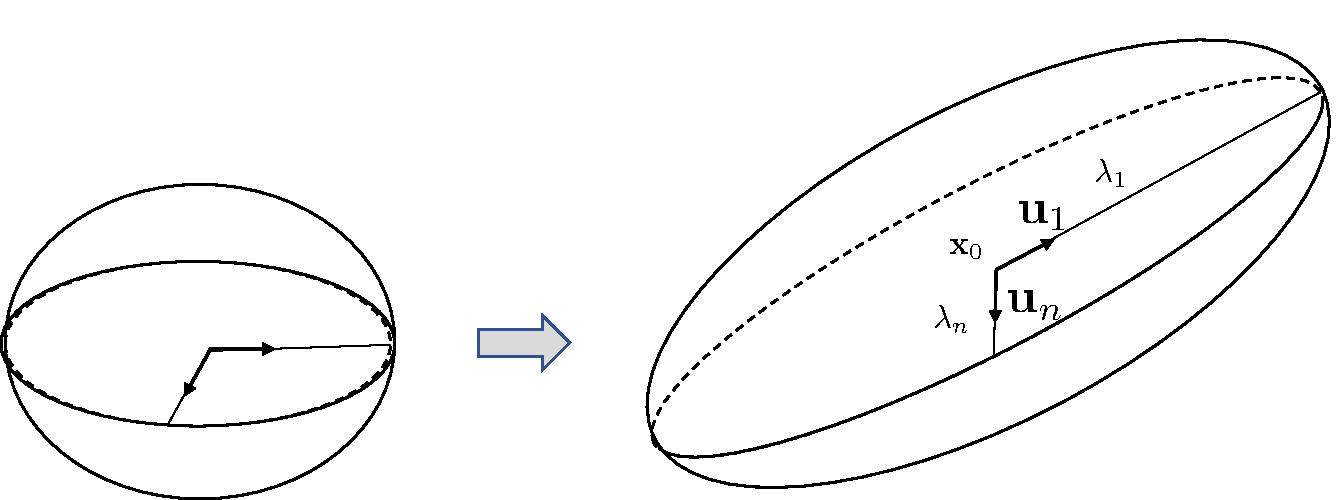
\includegraphics[width=0.6\textwidth]
			{figures/chap6_mapping_2}
	\end{center}
\end{frame}

%----------------------------------
\begin{frame}\frametitle{Quadratic Forms}
	We have essentially proved the following theorem:
	\begin{theorem}[Moon Theorem 6.5]
		For a positive semi-definite Hermitian matrix $A$, the maximum
		\[ 
			\lambda_1 = \max_{\norm{\xbf}_2=1} \xbf^H A \xbf 
		\]
		where $\lambda_1$ is the largest eigenvalue of $A$, and the maximizing $\xbf$ is $\xbf = \ubf_1$, the associated eigenvector.
		
		\vfill
		
		Furthermore if we maximize $\xbf^H A \xbf$ subject to the constraints
		\begin{align*}
			\iprod{\xbf, \ubf_i} &= 0 \qquad i = 1,\ldots,k-1, \\
			\norm{\xbf}_2 &= 1 
		\end{align*}
		then the maximum is $\lambda_k$ and $\xbf_{max} = \ubf_k$.		
	\end{theorem}
\end{frame}

%----------------------------------
\begin{frame}\frametitle{Quadratic Forms}
	Note that if $A$ is positive semi-definite Hermitian then
	\begin{align*}
		\norm{A}_2 
			= \sup_{\norm{\xbf}_2\neq 0}\frac{\norm{A\xbf}_2}{\norm{\xbf}_2} 
			= \max_{\norm{\xbf}_2 = 1} \sqrt{\xbf^H A^H A\xbf} 
			= \sqrt{\lambda_1 \ubf_1^H \ubf_1} 
			= \sqrt{\lambda_1} 
	\end{align*}
	where $\lambda_1$ is the largest eigenvalue of $A^H A$.
	
	\vfill
	
	More generally,
	\[ 
		R(x) = \frac{\xbf^\top A\xbf}{\xbf^\top \xbf} 
	\] 
	is called a Rayleigh quotient and
	\begin{align*}
		\max_{\norm{\xbf}\neq 0} R(\xbf) &= \lambda_1 \\
		\min_{\norm{\xbf}\neq 0} R(\xbf) &= \lambda_n.
	\end{align*}
\end{frame}




\end{document}